\chapter{Métodos de interpolación}
Con frecuencia se encontrará con que se tiene que estimar valores intermedios entre puntos asociados con datos. El método más común que se usa 
para este propósito es la interpolación polinomial. La fórmula general para un polinomio de n-ésimo grado es
\begin{equation}
	f(x) = a_0 + a_1x + a_2x^2 + \cdots + a_nx^n.
	\label{eq:polinomioInterpolacion}
\end{equation}
Dados $n+1$ puntos asociados con datos, hay uno y sólo un polinomio de grado $n$ que pasa a través de todos los puntos. La 
\textit{interpolación polinomial} consiste en determinar el polinomio único de $n$-ésimo grado que se ajuste a $n+1$ puntos asociados con datos. 
Este polinomio, entonces, proporciona una fórmula para calcular valores intermedios.

\section{Interpolación simple}
La forma más simple de interpolación es la que se conoce como \textit{interpolación lineal}. Esta técnica consiste en unir dos puntos asociados 
con datos con una línea recta. 

Sean los puntos $(x_0,f(x_0))$ y $(x_1,f(x_1))$, se puede construir un polinomio de primer grado calculando la pendiente entre los puntos:
\begin{align*}
	m &= \dfrac{y_2-y_1}{x_2-x_1} = \dfrac{f(x_1)-f(x_0)}{x_1-x_0}
\end{align*}
Ahora se construye un polinomio de primer grado con la ecuación \textit{punto-pendiente}:
\begin{align*}
	y-y_0 &= m(x-x_0)\\
	y-f(x_0) &= \dfrac{f(x_1)-f(x_0)}{x_1-x_0}(x-x_0)\\
	y &= f(x_0) + \dfrac{f(x_1)-f(x_0)}{x_1-x_0}(x-x_0)
\end{align*}
\begin{equation}
	f_1(x) = f(x_0) + \dfrac{f(x_1)-f(x_0)}{x_1-x_0}(x-x_0)
	\label{eq:interpolacionSimple}
\end{equation}

La expresión \ref{eq:interpolacionSimple} es una \textit{fórmula de interpolación lineal}, donde la notación $f_1(x)$ indica que se trata de 
un polinomio de primer grado.

\begin{example}{\rm
Estime el logaritmo natural de 2 mediante interpolación lineal. Utilice $\ln 1 = 0$ y $\ln 6 = 1.791759$. Repita el ejercicio utilizando 
ahora $\ln 1 = 0$ y $\ln 4 = 1.386294$.

\subsubsection*{Solución.} 

\begin{enumerate}[a)]
	\item Sea:
		\begin{align*}
			x_0 &= 1\\
			f(x_0) &= \ln 1\\
			x_1 &= 6 \\
			f(x_1) &= \ln 6
		\end{align*}
		\begin{align*}
			f_1(x) &= f(x_0) + \dfrac{f(x_1)-f(x_0)}{x_1-x_0}(x-x_0) \\
			f_1(2) &= \ln 1 + \dfrac{\ln 6 -\ln 1}{6-1} = 0.358351 \\
			\ln 2 &\approx 0.358351
		\end{align*}
		
	\item Sea:
		\begin{align*}
			x_0 &= 1\\
			f(x_0) &= \ln 1\\
			x_1 &= 4 \\
			f(x_1) &= \ln 4
		\end{align*}
		\begin{align*}
			f_1(x) &= f(x_0) + \dfrac{f(x_1)-f(x_0)}{x_1-x_0}(x-x_0) \\
			f_1(2) &= \ln 1 + \dfrac{\ln 4 -\ln 1}{4-1} =  \\
			\ln 2 &\approx 0.462098
		\end{align*}
\end{enumerate}
}\end{example}

\begin{example}{\rm 
Utilice los datos de la tabla \ref{table:ejemplo2InterpolacionSimple} para obtener una aproximación al valor de $f(1.5)$. 
Utilice la interpolación simple.
	
	\begin{table}[H]
		\centering
      \begin{tabular}{|c|c|}
				\hline 
				\rowcolor[gray]{0.9} $x$ & $f(x)$\\ \hline
					$1.0$ & $0.7651977$ \\
					$1.3$ & $0.6200860$ \\
					$1.6$ & $0.4554022$ \\
					$1.9$ & $0.2818186$ \\
					$2.2$ & $0.1103623$ \\
				\hline
      	\end{tabular}
      	\caption{Datos del Ejemplo \ref{ex:ejemplo2InterpolacionSimple}}
      	\label{table:ejemplo2InterpolacionSimple}
	\end{table}	
	
	\subsubsection*{Solución.} 
	Dado que el valor que se encontrará una aproximar se encuentra entre los valores $1.3$ y $1.6$, se utilizarán estos para realizar 
	la interpolación.
	\begin{align*}
		x_0 &= 1.3 \\
		f(x_0) &= 0.6200860\\
		x_1 &= 1.6 \\
		f(x_1) &= 0.4554022 \\
		f(x) &= 0.6200860 + \dfrac{0.4554022-0.6200860}{1.6-1.3}\cdot (1.5-1.3) = 0.5102968\\
		f(1.5) &\approx 0.5102968
	\end{align*}
	
	\label{ex:ejemplo2InterpolacionSimple}
}\end{example}

\section{Interpolación polinomial de Newton}
En la sección anterior utilizamos la interpolación para generar aproximaciones de primer grado. Los métodos de diferencias 
divididas, que explicaremos en esta sección, se usarán para generar sucesivamente los polinomios de grado $n$ por sí mismos.

\subsection{Diferencias Divididas}

Supongamos que $P_n(x)$ es el $n$-ésimo polinomio que concuerda con la función $f$ en los números distintos $x_0, x_1, \dots , x_n$. Dicho
polinomio $P_n(x)$ tiene la forma 
\begin{equation}
	P_n(x) = a_0 + a_1(x-x_0) + a_2(x-x_0)(x-x_1) + \cdots + a_n(x-x_0)\cdots (x-x_{n-1}),
	\label{eq:polinomioDiferenciasDivididas}
\end{equation}
para las constantes apropiadas $a_0, a_1, \dots ,a_n$. 

Para determinar la primera de las constantes $a_0$ se evalúa el polinomio $P_n$ de la ecuación \ref{eq:polinomioDiferenciasDivididas} en $x_0$, esto es:
$$P_n(x_0) = a_0 = f(x_0),$$
que a su vez debe ser igual a $f(x_0)$ dado que el polinomio $P_n$ debe coincidir con la función en $x_0$.

De manera similar, cuando se evalúa $P_n(x)$ en $x_1$, los únicos términos diferentes de cero en la evaluación de $P_n(x_1)$ son los términos 
constante y lineal,
$$P_n(x_1) = f(x_0) + a_1(x_1-x_0) = f(x_1);$$ 
de manera análoga se iguala con $f(x_1)$ y despejando el término $a_1$:
\begin{equation}
	a_1 = {f(x_1) - f(x_0)\over x_1 - x_0}
	\label{eq:segundoTerminoPolinomioDD}
\end{equation}

La expresión \ref{eq:segundoTerminoPolinomioDD} resulta ser la primer diferencia dividida.
De esta forma, reescribiendo los términos y generalizando se dice que la diferencia dividida cero de la función $f$ respecto a $x_1$  se denota como $f[x_i]$, 
esto es:
$$f[x_i] = f(x_i)$$
El resto de las diferencias divididas se definen en forma recursiva utilizando como base la expresión \ref{eq:segundoTerminoPolinomioDD}. De esta forma 
la \textit{primera diferencia dividida} de $f$ con respecto a $x_i$ y $x_{i+1}$ se denota:
$f[x_i, x_{i+1}]$ y se define así
\begin{equation}
	f[x_i, x_{i+1}] = {f[x_{i+1}] - f[x_i]\over x_{i+1} - x_i}.
	\label{eq:primeraDiferenciaDividida}
\end{equation}
La \textit{segunda diferencia dividida}, $f[x_i, x_{i+1}, x_{i+2}]$, se define como sigue
$$f[x_i, x_{i+1}, x_{i+2}] = {f[x_{i+1}, x_{i+2}] - f[x_i, x_{i+1}]\over x_{i+2} - x_i}$$
El proceso termina con la $n$-ésima diferencia dividida,
$$f[x_0, x_1, \dots, x_n] = {f[x_1, x_2, \dots , x_n] - f[x_0, x_1, \dots, x_{n-1}] \over x_n - x_0}$$
Por tanto el polinomio de interpolación en la ecuación \ref{eq:polinomioDiferenciasDivididas} es
$$P_n(x) = f[x_0] + f[x_0, x_1](x-x_0) + a_2(x-x_0)(x-x_1) + \cdots + a_n(x-x_0)(x-x_1)\cdots (x-x_{n-1}).$$
Podemos reescribir $P_n(x)$ en una forma llamada diferencia dividida de Newton:
\begin{equation}
	P_n(x) = f[x_0] + \sum_{k=1}^n f[x_0, x_1, \dots , x_k](x-x_0)\dots (x-x_{k-1}).
	\label{eq:diferenciaDivididaNewton}
\end{equation}
El valor de $f[x_0, x_1, \dots, x_k]$ es independiente del orden de los números $x_0, x_1, \dots, x_k$.


\begin{theorem}[Diferencias divididas de Newton]
	\[P_n(x) = F_{0,0} + \sum_{i=1}^n F_{i,i} \prod_{j=0}^{i-1}(x-x_j).\]
	donde $F_{i,i}$ es $f[x_0,x_1,\dots,x_i]$.
\end{theorem}

\begin{algorithm}[ht]
  	\SetKwInOut{Input}{Entrada}
  	\SetKwInOut{Output}{Salida}
  	\SetKwFunction{Salida}{Salida}
  	\Input{Números $x_0,x_1,\dots,x_n$; valores $f(x_0), f(x_1),\dots, f(x_n)$ como $F_{0,0}, F_{1,0},\dots, F_{n,0}$.}
	\Output{Los números $F_{0,0}, F_{1,1}, \dots , F_{n,n}$ donde\\
	$$P_n(x) = F_{0,0} + \sum_{i=1}^n F_{i,i} \prod_{j=0}^{i-1}(x-x_j).$$
	$$(F_{i,i})\, es\, f[x_0,x_1,\dots,x_i].$$}
	\Begin{
		\For{$i=1$ \KwTo $n$}{
			\For{$j=1$ \KwTo $i$}{
				$F_{i,j} = \displaystyle{F_{i,j-1} - F_{i-1,j-1}\over x_i - x_{i-j}}$
			}	
		}
		\Salida($F_{0,0}, F_{1,1}, \dots, F_{n,n}$;)
  	}
	\caption{Diferencias Divididas de Newton}
	\label{algo:diferenciasDivididasNewton}
\end{algorithm}


\begin{example}
\label{ex:ejemplo1DiferenciasDivididasNewton}
{\rm Con los datos de la tabla \ref{table:ejemplo1ADiferenciasDivididasNewton} construya el 
		polinomio de interpolación de mayor grado posible. Utilizando el polinomio resultante, aproxime $P(1.5)$.
	
	\begin{table}[H]
		\label{table:ejemplo1ADiferenciasDivididasNewton}
		\centering
      \begin{tabular}{|c|c|}
				\hline 
				\rowcolor[gray]{0.9} $x$ & $f(x)$\\ \hline
					$1.0$ & $0.7651977$ \\
					$1.3$ & $0.6200860$ \\
					$1.6$ & $0.4554022$ \\
					$1.9$ & $0.2818186$ \\
					$2.2$ & $0.1103623$ \\
				\hline
      	\end{tabular}
      	\caption{Datos del Ejemplo \ref{ex:ejemplo1DiferenciasDivididasNewton}}
	\end{table}	
	
	\subsubsection*{Solución.} La primera diferencia dividida que involucra a $x_0$ y $x_1$ es
		$$f[x_0,x_1] = {f[x_1] - f[x_0]\over x_1 - x_0} = {0.6200860-0.7651877\over 1.3-1.0} = -0.4837057.$$
		El resto de las primeras diferencias divididas se calcularon de manera similar y se muestran el la cuarta columna de la tabla
		\ref{table:ejemplo1BDiferenciasDivididasNewton}.
	
	\begin{table}[H]
		\centering
      \begin{tabular}{|c|c|c|c|c|c|c|}
				\hline 
				\rowcolor[gray]{0.9} $i$ & $x_i$ & $f[x_i]$ & $f[x_{i-1}, x_i]$ & $f[x_{i-2},x_{i-1},x_i]$ & $f[x_{i-3},\dots,x_i]$ & $f[x_{i-4},\dots, x_i]$\\
				 \hline
					0 & $1.0$ & $0.7651977$ & & & & \\ 
						&&&$-0.4837057$&&&\\
					1 & $1.3$ & $0.6200860$ &  & $-0.1087339$ & & \\
						&&&$-0.5489460$&&$0.0658784$&\\
					2 & $1.6$ & $0.4554022$ &  & $-0.0494433$ & & $0.0018251$\\
						&&&$-0.5786120$&&$0.0680685$&\\
					3 & $1.9$ & $0.2818186$ &  & $ 0.0118183$ &  & \\
						&&&$-0.5715210$&&&\\
					4 & $2.2$ & $0.1103623$ &  &  &  &  \\
				\hline
      	\end{tabular}
      	\caption{Diferencias Divididas del Ejemplo \ref{ex:ejemplo1DiferenciasDivididasNewton}}
      	\label{table:ejemplo1BDiferenciasDivididasNewton}
	\end{table}
	
	La segunda diferencia dividida que implica a $x_0, x_1$ y $x_2$ es
	$$f[x_0,x_1,x_2] = {f[x_1,x_2]-f[x_0-x_1]\over x_2-x_0} = {-0.5489460-(-0.4837057)\over 1.6 - 1.0} = -0.1087339$$
	La segunda diferencia dividida restante se muestra en la quinta columna de la tabla \ref{table:ejemplo1BDiferenciasDivididasNewton}. La tercera diferencia
	dividida que involucra a $x_0, x_1, x_2$ y $x_3$ y la cuarta diferencia dividida que involucra todos los puntos existentes son, respectivamente,
	$$f[x_0,x_1,x_2,x_3] = {f[x_1,x_2,x_3]-f[x_0,x_1,x_2]\over x_3-x_0} = {-0.0494433-(-0.1087339)\over 1.9-1.0} = 0.0658784,$$
	y
	$$f[x_0,x_1,x_2,x_3,x_4] = {f[x_1,x_2,x_3,x_4]-f[x_0,x_1,x_2,x_3]\over x_4-x_0} = {0.0680685-0.0658784\over 2.2-1.0} = 0.0018251.$$
	Los coeficientes de la fórmula de las diferencias divididas del polinomio de interpolación de Newton se encuentran a lo largo de la diagonal 
	de la tabla \ref{table:ejemplo1BDiferenciasDivididasNewton}. Por lo tanto, el polinomio es
	$$P_4(x) = 0.7651977 - 0.4837057\cdot(x-1.0) - 0.1087339\cdot(x-1.0)(x-1.3) + $$
	$$0.0658784\cdot(x-1.0)(x-1.3)(x-1.6) + 0.0018251\cdot(x-1.0)(x-1.3)(x-1.6)(x-1.9)$$
	Finalmente la aproximación es:
	$$P_4(1.5) = 0.7651977 - 0.4837057\cdot(1.5-1.0) - 0.1087339\cdot(1.5-1.0)(1.5-1.3) + $$
	$$0.0658784\cdot(1.5-1.0)(1.5-1.3)(1.5-1.6) + 0.0018251\cdot(1.5-1.0)(1.5-1.3)(1.5-1.6)(1.5-1.9)$$
	$$P_4(1.5) = 0.5118200$$ 
}\end{example}
\hrulefill\\

\begin{example}{\rm Construya el polinomio de aproximación de mayor grado posible para los siguientes datos: $f(8.1)=16.94410$, $f(8.3)=17.56492$,
		$f(8.6)=18.50515$ y $f(8.7)=18.82091$. Use el polinomio para aproximar a $f(8.4)$.\\
	\subsubsection*{Solución.} 
		Calculamos las primeras diferencias divididas.
		$$f[x_0,x_1] = {f[x_1] - f[x_0]\over x_1 - x_0} = {17.56492-16.94410\over 8.3-8.1} = 3.1041.$$
		$$f[x_1,x_2] = {f[x_2] - f[x_1]\over x_2 - x_1} = {18.50515-17.56492\over 8.6-8.3} = 3.1341.$$
		$$f[x_2,x_3] = {f[x_3] - f[x_2]\over x_3 - x_2} = {18.82091-18.50515\over 8.7-8.7} = 3.1576.$$
		Ahora las segundas diferencias divididas.
		$$f[x_0,x_1,x_2] = {f[x_1,x_2] - f[x_0-x_1]\over x_2 - x_0} = {3.1341-3.1041\over 8.6-8.1} = 0.06.$$
		$$f[x_1,x_2,x_3] = {f[x_2,x_3] - f[x_1,x_2]\over x_3 - x_1} = {3.1576-3.1341\over 8.7-8.3} = 0.05875.$$
		La tercera y última diferencia dividida.
		$$f[x_0,x_1,x_2,x_3] = {f[x_1,x_2,x_3]-f[x_0,x_1,x_2]\over x_3-x_0} = {0.058750-0.06\over 8.7-8.1} = -0.00208333$$
	Todos los resultados anteriores los concentramos en la tabla \ref{table:ejemplo2DiferenciasDivididasNewton}.
	\begin{table}[H]
		\centering
      \begin{tabular}{|c|c|c|c|c|c|}
				\hline 
				\rowcolor[gray]{0.9} $i$ & $x_i$ & $f[x_i]$ & $f[x_{i-1}, x_i]$ & $f[x_{i-2},x_{i-1},x_i]$ & $f[x_{i-3},\dots,x_i]$\\ \hline
					0 & $8.1$ & $16.94410$ & & & \\
					1 & $8.3$ & $17.56492$ & $3.1041$ &  & \\
					2 & $8.6$ & $18.50515$ & $3.1341$ & $0.06$ & \\
					3 & $8.7$ & $18.82091$ & $3.1576$ & $0.058750$ & $-0.00208333$ \\
				\hline
      	\end{tabular}
      	\caption{Diferencias Divididas del Ejemplo \ref{ex:ejemplo2DiferenciasDivididasNewton}}
      	\label{table:ejemplo2DiferenciasDivididasNewton}
	\end{table}

	Los coeficientes de la fórmula de las diferencias divididas del polinomio de interpolación de Newton se encuentran a lo largo de la diagonal 
	de la tabla \ref{table:ejemplo2DiferenciasDivididasNewton}. Por lo tanto, el polinomio es
	$$P_3(x) = 16.94410 + 3.1041\cdot(x-8.1) + 0.06\cdot(x-8.1)(x-8.3) - $$
	$$0.00208333\cdot(x-8.1)(x-8.3)(x-8.6)$$	
	Finalmente la aproximación es:
	$$P_3(8.4) = 16.94410 + 3.1041\cdot(8.4-8.1) + 0.06\cdot(8.4-8.1)(8.4-8.3) - $$
	$$0.00208333\cdot(8.4-8.1)(8.4-8.3)(8.4-8.6) = 17.8771175$$
	
	\label{ex:ejemplo2DiferenciasDivididasNewton}
}\end{example}

%\section{Interpolación de Punto Fijo}

\section{Interpolación de Lagrange}
El problema de definir un polinomio de primer grado que pasa por los puntos distintos $(x_0, y_0)$ y $(x_1, y_1)$ es el mismo que el de 
aproximar una función $f$, para la cual $f(x_0) = y_0$ y $f(x_1) = y_1$ por medio de un polinomio de primer grado que \textbf{interpole} 
los valores de $f$ en los puntos dados o que coincida con ellos. Este procedimiento utilizado para aproximar dentro del intervalo dado 
por los extremos es llamado polinomio de \textbf{interpolación}.

Definamos las funciones 

\begin{center}
	$L_0 = \displaystyle{x - x_1\over x_0 - x_1}$ y $L_1 = \displaystyle{x - x_0\over x_1 - x_0}$.
\end{center}

El polinomio de interpolación de Lagrange lineal que pasa por $(x_0, y_0)$ y $(x_1, y_1)$ es
$$P(x) = L_0(x)f(x_0) + L_1(x)f(x_1) = {x - x_1\over x_0 - x_1}f(x_0) + {x - x_0\over x_1 - x_0}f(x_1).$$
Observe que

\begin{center}
	$L_0(x_0) = 1$, $L_0(x_1) = 0$, $L_1(x_0) = 0$ y $L_1(x_1) = 1$
\end{center}

lo cual implica que 
$$P(x_0) = 1\cdot f(x_0) + 0\cdot f(x_1) = f(x_0) = y_0$$
y
$$P(x_1) = 0\cdot f(x_0) + 1\cdot f(x_1) = f(x_1) = y_1$$
Así $P$ es el único polinomio de primer grado como máximo que pasa por $(x_0, y_0)$ y $(x_1, y_1)$.

\begin{example}{\rm 
	Determine el polinomio de interpolación lineal de Lagrange que pasa por los puntos $(2, 4)$ y $(5, 1)$.\\
	\subsubsection*{Solución.} En este caso tenemos
		$$L_0(x) = {x-5\over 2-5} = -\frac{1}{3}(x-5)$$	
		y
		$$L_1(x) = {x-2\over 5-2} = \frac{1}{3}(x-2)$$
		por lo que
		$$P(x) = -\frac{1}{3}(x-5)\cdot 4 + \frac{1}{3}(x-2)\cdot 1 = -\frac{4}{3}x + \frac{20}{3} + \frac{1}{3}x - \frac{2}{3} = -x + 6$$
}\end{example}

A fin de generalizar el concepto a partir de la interpolación lineal, consideremos la construcción de un polinomio de grado máximo $n$ 
que pase por los $n+1$ puntos
$$\{(x_0, f(x_0)), (x_1, f(x_1)), \dots ,(x_n, f(x_n))\}.$$

En este caso para cada $k=0,1, \dots , n$ construimos una función $L_{n,k}(x)$ con la propiedad de que $L_{n,k}(x_i) = 0$, 
cuando $i\not= k$ y $L_{n,k}(x_i) = 1$.
Para satisfacer $L_{n,k}(x_i) = 0$ para cada $i\not= k$ se requiere que el numerador de $L_{n,k}(x)$ contenga el término
$$(x-x_0)(x-x_1)\cdots (x-x_{k-1})(x-x_{k+1})\cdots (x-x_n).$$
Para satisfacer $L_{n,k}(x_k) = 1$, el denominador de $L_{n,k}(x)$ debe ser este término pero evaluado en $x=x_k$; es decir,
$$L_{n,k}(x) = {(x-x_0)(x-x_1)\cdots (x-x_{k-1})(x-x_{k+1})\cdots (x-x_n) \over (x_k-x_0)(x_k-x_1)\cdots (x_k-x_{k-1})(x_k-x_{k+1})\cdots (x_k-x_n)}.$$

El polinomio de interpolación se describe fácilmente ahora que conocemos la forma de $L_{n,k}$. Este polinomio, denominado 
\textbf{$\textbf{n}$-ésimo polinomio de interpolación de Lagrange}, se describe en el siguiente teorema.

\begin{theorem}[Teorema de polinomio de Lagrange]
	Si $x_0, x_1, \dots , x_n$ son $n+1$ números distintos y si $f$ es una función cuyos valores están dados en estos números, entonces existe 
	un único polinomio $P(x)$ de grado máximo $n$, con la propiedad de que
	$$f(x_k) = P(x_k),\, \forall k=0,1,\dots , n.$$	
	Este polinomio está dado por
	
	\begin{equation}
		P(x) = f(x_0)L_{n,0}(x) + \cdots + f(x_n)L_{n,n}(x) = \sum_{k=0}^n f(x_k)L_{n,k}(x)
		\label{eq:polinomioLagrange}
	\end{equation}
	
	donde, para cada $k=0,1,\dots , n,$
	\begin{equation}
		L_{n,k}(x) = {(x-x_0)(x-x_1)\cdots (x-x_{k-1})(x-x_{k+1})\cdots (x-x_n) \over (x_k-x_0)(x_k-x_1)\cdots (x_k-x_{k-1})(x_k-x_{k+1})\cdots (x_k-x_n)} \\
		= \prod_{i=0, i\not= k}^{n} {(x-x_i) \over (x_k - x_i)}. 
		\label{eq:coeficientesLagrange}
	\end{equation}
\end{theorem}

Escribiremos $L_{n,k}(x)$ simplemente como $L_{k}(x)$ cuando no hay confusión respecto a su grado.

\begin{example}{\rm 
		\begin{enumerate}[a)]
			\item Utilice los números (o nodos) $x_0 = 2$, $x_1 = 2.75$ y $x_2 = 4$ para obtener el segundo polinomio de interpolación de 
				Lagrange para $f(x) = 1/x$.
			\item Use este polinomio para aproximar $f(3) = 1/3$.
		\end{enumerate}
		\subsubsection*{Solución.}
		\begin{enumerate}[a)]
			\item Primero determinamos los polinomios de coeficientes $L_0(x)$, $L_1(x)$ y $L_2(x)$. 
				Dado que $n=2$, los coeficientes de Lagrange de la expresión \ref{eq:coeficientesLagrange} se reducen a:
				$$L_{2,0}(x) = L_0(x) = \prod_{i=0, i\not= 0}^{2} {(x-x_i) \over (x_0 - x_i)} = {(x-x_1)(x-x_2)\over (x_0-x_1)(x_0-x_2)}$$	
				$$L_{2,1}(x) = L_1(x) = \prod_{i=0, i\not= 1}^{2} {(x-x_i) \over (x_1 - x_i)} = {(x-x_0)(x-x_2)\over (x_1-x_0)(x_1-x_2)}$$	
				$$L_{2,2}(x) = L_2(x) = \prod_{i=0, i\not= 2}^{2} {(x-x_i) \over (x_2 - x_i)} = {(x-x_0)(x-x_1)\over (x_2-x_0)(x_2-x_1)}$$	
				En forma anidada son
				$$L_0(x) = {(x-2.75)(x-4)\over (2-2.75)(2-4)} = \frac{2}{3}(x-2.75)(x-4),$$
				$$L_1(x) = {(x-2)(x-4)\over (2.75-2)(2.75-4)} = -\frac{16}{15}(x-2)(x-4),$$
				y
				$$L_2(x) = {(x-2)(x-2.75)\over (4-2)(4-2.75)} = \frac{2}{5}(x-2)(x-2.75).$$		
				Puesto que $f(x_0) = f(2) = 1/2$, $f(x_1) = f(2.75) = 4/11$ y $f(x_2) = f(4) = 1/4$, tenemos
				$$P(x) = \sum_{k=0}^2 f(x_k)L_k(x) =  \frac{1}{2}\cdot\frac{2}{3}(x-2.75)(x-4) + \frac{4}{11}\cdot\left(-\frac{16}{15}\right)(x-2)(x-4) + 
				\frac{1}{4}\cdot\frac{2}{5}(x-2)(x-2.75) $$
				$$ = \frac{1}{3}(x-2.75)(x-4) - \frac{64}{165}(x-2)(x-4) + \frac{1}{10}(x-2)(x-2.75)$$
				$$ = \frac{1}{22}x^2 - \frac{35}{88}x + \frac{49}{44}.$$
			\item Una aproximación a $f(3) = 1/3$ es
				$$f(3) \approx P(3) = \frac{9}{22} - \frac{105}{88} + \frac{49}{44} = \frac{29}{88} \approx 0.32955.$$
		\end{enumerate}
}\end{example}


\begin{example}{\rm Para la función dada $f(x) = \sin (\pi x)$, sean $x_0=1$, $x_1=1.25$ y $x_2=1.6$. Construya el polinomio de interpolación 
de segundo grado para aproximar $f(1.4)$, y calcule el error máximo.\\
	\subsubsection*{Solución.} Dado que $n=2$, los coeficientes de Lagrange $L_0(x)$, $L_1(x)$ y $L_2(x)$ de la expresión \ref{eq:coeficientesLagrange} son:
			$$L_0(x) = \prod_{i=0, i\not= 0}^{2} {(x-x_i) \over (x_0 - x_i)} = {(x-x_1)(x-x_2)\over (x_0-x_1)(x_0-x_2)}$$	
			$$L_1(x) = \prod_{i=0, i\not= 1}^{2} {(x-x_i) \over (x_1 - x_i)} = {(x-x_0)(x-x_2)\over (x_1-x_0)(x_1-x_2)}$$	
			$$L_2(x) = \prod_{i=0, i\not= 2}^{2} {(x-x_i) \over (x_2 - x_i)} = {(x-x_0)(x-x_1)\over (x_2-x_0)(x_2-x_1)}$$	
		Sustituyendo los datos del problema:
			$$L_0(x) = {(x-1.25)(x-1.6)\over (1-1.25)(1-1.6)} = \frac{20}{3}(x-1.25)(x-1.6) = \frac{20}{3}x^2 - 19x + \frac{40}{3}$$
			$$L_1(x) = {(x-1)(x-1.6)\over (1.25-1)(1.25-1.6)} = -\frac{80}{7}(x-1)(x-1.6) = -\frac{80}{7}x^2 + \frac{208}{7}x - \frac{128}{7}$$
			$$L_2(x) = {(x-1)(x-1.25)\over (1.6-1)(1.6-1.25)} = \frac{100}{21}(x-1)(x-1.25) = \frac{100}{21}x^2 - \frac{75}{7}x + \frac{125}{21}$$
		Sustituyendo los puntos en la función dada:
			$$f(x_0) = f(1) = \sin (\pi) = 0$$
			$$f(x_1) = f(1.25) = \sin (1.25\pi) = -\frac{1}{\sqrt{2}}$$
			$$f(x_2) = f(1.6) = \sin (1.6\pi) = -0.951057$$
		Formando el Polinomio de Lagrange
			$$P(x) = \sum_{k=0}^2 f(x_k)L_{2,k}(x) = f(x_0)L_0(x) + f(x_1)L_1(x) + f(x_2)L_2(x)$$
			$$P(x) = 0\cdot \left[ \frac{20}{3}x^2 - 19x + \frac{40}{3} \right] - \frac{1}{\sqrt{2}}\cdot \left[-\frac{80}{7}x^2 + \frac{208}{7}x 
			- \frac{128}{7}\right]
			-0.951057\cdot \left[ \frac{100}{21}x^2 - \frac{75}{7}x + \frac{125}{21} \right]$$
			$$P(x) = 3.55238x^2 - 10.8213x + 7.2689$$
		Calculando la aproximación al punto $x=1.4$
			$$P(1.4) = 3.55238(1.4)^2 - 10.8213(1.4) + 7.2689 \approx -0.91826$$
}\end{example}

\begin{example}{\rm Use el polinomio de interpolación de Lagrange apropiados de grado tres para aproximar lo siguiente: $f(8.4)$ si 
	$f(8.1)=16.94410$, $f(8.3)=17.56492$, $f(8.6)=18.50515$, $f(8.7)=18.82091$.
	\subsubsection*{Solución.} Dado que $n=3$, es necesario encontrar los coeficientes $L_0(x)$, $L_1(x)$, $L_2(x)$ y $L_3(x)$. 
	La expresión \ref{eq:coeficientesLagrange} 
		se reduce a:
			$$L_0(x) = \prod_{i=0, i\not= 0}^{2} {(x-x_i) \over (x_0 - x_i)} = {(x-x_1)(x-x_2)(x-x_3)\over (x_0-x_1)(x_0-x_2)(x_0-x_3)}$$	
			$$L_1(x) = \prod_{i=0, i\not= 1}^{2} {(x-x_i) \over (x_1 - x_i)} = {(x-x_0)(x-x_2)(x-x_3)\over (x_1-x_0)(x_1-x_2)(x_1-x_3)}$$	
			$$L_2(x) = \prod_{i=0, i\not= 2}^{2} {(x-x_i) \over (x_2 - x_i)} = {(x-x_0)(x-x_1)(x-x_3)\over (x_2-x_0)(x_2-x_1)(x_2-x_3)}$$
			$$L_3(x) = \prod_{i=0, i\not= 3}^{2} {(x-x_i) \over (x_3 - x_i)} = {(x-x_0)(x-x_1)(x-x_2)\over (x_3-x_0)(x_3-x_1)(x_3-x_2)}$$
		Sustituyendo las coordenadas dadas por el problema:
			$$L_0(x) = {(x-8.3)(x-8.6)(x-8.7)\over (8.1-8.3)(8.1-8.6)(8.1-8.7)} = {(x-8.3)(x-8.6)(x-8.7)\over -(\frac{1}{5})(\frac{1}{2})(\frac{3}{5})}$$
			$$L_0(x) = -\frac{50}{3}(x-8.3)(x-8.6)(x-8.7)$$
			$$L_1(x) = {(x-8.1)(x-8.6)(x-8.7)\over (8.3-8.1)(8.3-8.6)(8.3-8.7)} = {(x-8.1)(x-8.6)(x-8.7)\over (\frac{1}{5})(-\frac{3}{10})(-\frac{2}{5})}$$
			$$L_1(x) = \frac{250}{6}(x-8.1)(x-8.6)(x-8.7)$$
			$$L_2(x) = {(x-8.1)(x-8.3)(x-8.7)\over (8.6-8.1)(8.6-8.3)(8.6-8.7)} = {(x-8.1)(x-8.3)(x-8.7)\over (\frac{1}{2})(\frac{3}{10})(-\frac{1}{10})}$$
			$$L_2(x) = -\frac{200}{3}(x-8.1)(x-8.3)(x-8.7)$$
			$$L_3(x) = {(x-8.1)(x-8.3)(x-8.6)\over (8.7-8.1)(8.7-8.3)(8.7-8.6)} = {(x-8.1)(x-8.3)(x-8.6)\over (\frac{3}{5})(\frac{2}{5})(\frac{1}{10})}$$
			$$L_3(x) = \frac{250}{6}(x-8.1)(x-8.3)(x-8.6)$$	
		Luego, sustituyendo estos coeficientes en el polinomio de Lagrange (ecuación \ref{eq:polinomioLagrange}) cuando $n=3$:
			$$P(x) = \sum_{k=0}^3 f(x_k)L_{3,k}(x) = f(x_0)L_0(x) + f(x_1)L_1(x) + f(x_2)L_2(x) + f(x_3)L_3(x)$$
			$$P(x) = (16.9441)\left[-\frac{50}{3} (x-8.3)(x-8.6)(x-8.7) \right] + (17.56492)\left[\frac{250}{6} (x-8.1)(x-8.6)(x-8.7) \right]$$
			$$+ (18.50515)\left[-\frac{200}{3} (x-8.1)(x-8.3)(x-8.7) \right] + (18.82091)\left[\frac{250}{6} (x-8.1)(x-8.3)(x-8.6) \right]$$
			$$P(x) = -0.0020833x^3 + 0.112083x^2 + 1.6861x - 2.96077$$
		Finalmente sustituyendo $x=8.4$ para obtener la aproximación
			$$P(8.4) = -0.0020833(8.4)^3 + 0.112083(8.4)^2 + 1.6861(8.4) - 2.96077 = 17.8771062368$$
		Dado que se cumple que $f(8.3)\leq P(8.4)\leq f(8.6)$, es decir, $17.56492 \leq 17.8771062368 \leq 18.50515$ la aproximación es válida y apropiada.
		
}\end{example}


\section{Interpolación de mínimos cuadrados}

Considere el problema de encontrar un polinomio que se aproxime a un conjunto de datos obtenidos experimentalmente.
Se desea que el polinomio sea lo más próximo posible a los datos de manera que el error en la aproximación sea mínimo.  
Véase la figura \ref{fig:minimosCuadrados1} que muestra una gráfica de valores $x$ y $y$. 

\begin{figure}[H]
  \centering
  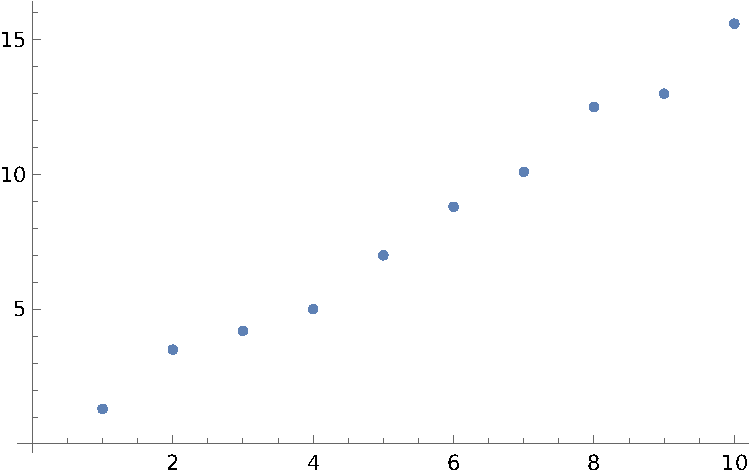
\includegraphics[scale=1]{img/minimosCuadradosLineales1.pdf}
  \caption{Gráfica de puntos Experimentales}
  \label{fig:minimosCuadrados1}
\end{figure}

De acuerdo a los datos que se encuentran en la figura \ref{fig:minimosCuadrados1}, es posible construir un polinomio de grado $n$, 
mostrado en la expresión \ref{eq:polinomioMinimosCuadrados}. 

\begin{equation}
	P_n(x) = a_0 + a_1x + a_2x^2 + \dots + a_nx^n
	\label{eq:polinomioMinimosCuadrados}
\end{equation}
Es natural que mientras sea mayor el grado del polinomio, mejor será la aproximación al conjunto de datos. En general, con una cantidad
de $m$ datos se puede construir un polinomio de grado máximo $n-2$. Esto es:

\[ n_{max} < m-1 \]

\subsection{Caso lineal}

El problema de determinar la ecuación de la mejor aproximación lineal en el sentido absoluto consiste en hallar los valores de $a_0$
y $a_1$ que minimicen

$$E_1(a_0, a_1) = \max_{1\leq i\leq m} \{|y_i - (a_1x_i + a_0)|\}.$$

A lo anterior comúnmente se le llama problema de \textbf{minimax} y no se puede resolver mediante métodos elementales.
Otro método para determinar la mejor aproximación lineal implica hallar los valores de $a_0$ y $a_1$ que minimicen

$$E_1(a_0, a_1) = \sum_{i=1}^m |y_i - (a_1x_i + a_0)|$$

Esta cantidad se llama \textbf{desviación absoluta}. Para minimizar una función de dos variables, necesitamos igualar a cero sus 
derivadas parciales y resolver en forma simultánea las ecuaciones resultantes. En el caso de la desviación absoluta, necesitamos hallar
$a_0$ y $a_1$ tales que 


	$$0 = \displaystyle{\dfrac{\delta}{\delta a_0} \sum_{i=1}^m |y_{i} - (a_1 x_i + a_0)|}$$
	$$0 = \displaystyle{\dfrac{\delta}{\delta a_1} \sum_{i=1}^m |y_{i} - (a_1 x_i + a_0)|}$$

El problema radica en que la función valor absoluto no es derivable en cero y no seríamos capaces de obtener las soluciones de este par
de ecuaciones.

El método de mínimos cuadrados para resolver este problema requiere determinar la mejor linea de aproximación cuando el error involucrado
es la suma de los cuadrados de las diferencias entre los valores de $y$ en la línea de aproximación y los valores de $y$ dados. Por tanto,
hay que encontrar las constantes $a_0$ y $a_1$ que reduzcan al mínimo el error de mínimos cuadrados:

$$E_2(a_0, a_1) = \sum_{i=1}^m \left[ y_i - (a_1x_i + a_0) \right]^2.$$

Para el calculo del error se utiliza la diferencia de cada punto con su aproximación. 
La idea es que cuando se eleva al cuadrado, las diferencias pequeñas se harán más pequeñas y las diferencias grandes se harán más grandes, 
por lo que el resultado final del error será en su mayoría obtenido por los puntos más lejanos de la aproximación.

El problema general de ajustar la mejor recta con mínimos cuadrados a una colección de datos $\{(x_i, y_i)\}_{i=1}^{m}$ implica minimizar
el error total,

$$E\equiv E_2(a_0, a_1) = \sum_{i=1}^{m} \left[ y_i - (a_1x_i + a_0) \right]^2,$$

con respecto a los parámetros $a_0$ y $a_1$. Para que haya un mínimo, debemos tener

\begin{center}
	$\displaystyle{\dfrac{\delta E}{\delta a_0}} = 0$\\ y $\displaystyle{\dfrac{\delta E}{\delta a_1}} = 0,$
\end{center}

esto es,

$$0 = \dfrac{\delta}{\delta a_0}\sum_{i=1}^{m} \left[ y_i - (a_1x_i + a_0) \right]^2 = 2\sum_{i=1}^{m} (y_i - a_1x_i - a_0)(-1)$$

y

$$0 = \dfrac{\delta}{\delta a_1}\sum_{i=1}^{m}\left[ y_i - (a_1x_i + a_0) \right]^2 = 2\sum_{i=1}^{m} (y_i - a_1x_i - a_0)(-x_i).$$

Estas ecuaciones se simplifican en las \textbf{ecuaciones normales}:

$$a_0\cdot m + a_1\sum_{i=1}^{m}x_i = \sum_{i=1}^{m}y_i
\,\wedge\,
a_0\sum_{i=1}^{m}x_i + a_{1}\sum_{i=1}^{m}x_i^2 = \sum_{i=1}^{m}x_iy_i.$$

La solución a este sistema de ecuaciones es:

\begin{equation}
	a_0 = \dfrac{\sum_{i=1}^{m}x_i^2 \sum_{i=1}^{m}y_i - \sum_{i=1}^{m}x_iy_i \sum_{i=1}^m x_i}{m \left(\displaystyle{\sum_{i=1}^{m}x_i^2}\right) - 
	\left(\displaystyle{\sum_{i=1}^m x_i}\right)^2}
	\label{eq:minimosCuadrados1}
\end{equation}

y

\begin{equation}
	a_1 = \dfrac{m\sum_{i=1}^{m}x_iy_i - \sum_{i=1}^{m}x_i \sum_{i=1}^m y_i}{m \left(\displaystyle{\sum_{i=1}^{m}x_i^2}\right) - 
	\left(\displaystyle{\sum_{i=1}^m x_i}\right)^2}
	\label{eq:minimosCuadrados2}
\end{equation}

Una vez calculados los valores de $a_0$ y $a_1$, la recta aproximada a los puntos es:

\begin{equation}
	P(x) = a_1x+a_0
	\label{eq:minimosCuadrados3}
\end{equation}

\begin{example}{\rm Obtenga la línea de mínimos cuadrados que aproxima a los datos de la tabla \ref{table:ejemplo1MinimosCuadradosLineales}.
	Utilice el polinomio para encontrar la aproximación $P(6)$.
	\subsubsection*{Solución.} 
	Primero se extiende la tabla con los valores experimentales agregando tres columnas. Dos de ellas tendrán
	el resultado de las operaciones $x_i^2$ y $x_iy_i$. La tercera columna se llena al final, después de calcular el valor de $a_0$
	y $a_1$. Esta columna contiene el valor de la línea de aproximación para cada punto experimental.
	\begin{table}[H]
    	\centering
      \begin{tabular}{|r|r|r|r|c|}
		\hline
		\rowcolor[gray]{0.9} $x_i$ & $y_i$ & $x_i^2$ & $x_iy_i$ & $P(x_i) = 1.538x_i - 0.360$\\\hline
			1 & 1.3 & 1 & 1.3 & 1.18\\
			2 & 3.5 & 4 & 7.0 & 2.72\\
			3 & 4.2 & 9 & 12.6 & 4.25\\
			4 & 5.0 & 16 & 20.0 & 5.79\\
			5 & 7.0 & 25 & 35.0 & 7.33\\
			6 & 8.8 & 36 & 52.8 & 8.87\\
			7 & 10.1 & 49 & 70.7 & 10.41\\
			8 & 12.5 & 64 & 100.0 & 11.94\\
			9 & 13.0 & 81 & 117.0 & 13.48\\
			10 & 15.6 & 100 & 156.0 & 15.02\\\hline
			55 & 81.0 & 385 & 572.4 & $E=\sum_{i=1}^{10} (y_i-P(x_i))^2 \approx 2.34$\\
		\hline
      \end{tabular}
      \label{table:ejemplo1MinimosCuadradosLineales}
      \caption{Valores experimentales}
  \end{table} 	
	
	Las ecuaciones normales \ref{eq:minimosCuadrados1} y \ref{eq:minimosCuadrados2} implican que
	\begin{align*}
		a_0 &= \dfrac{385(81) - 55(572.4)}{10(385) - (55)^2} = -0.360 \\
		a_1 &= \dfrac{10(572.4) - 55(81)}{10(385) - (55^2)} = 1.538
	\end{align*}
	por lo que la ecuación de la aproximación lineal por mínimos cuadrados \ref{eq:minimosCuadrados3} queda:
	\begin{align*}
		P(x)= 1.538x - 0.360
	\end{align*}
	Ahora se encuentra la evaluación:
	\begin{align*}
		P(6) &= 1.538(6) - 0.360 = 8.868.
	\end{align*}
	Este valor es consistente con los datos contenidos en la tabla \ref{table:ejemplo1MinimosCuadradosLineales}.
}\end{example}

\subsection{Caso no lineal}
El problema general de aproximar un conjunto de datos $\{(x_i, y_i)| i=1,2,\dots,m\}$, con un polinomio algebraico

$$P_n(x) = a_nx^n + a_{n-1}x^{n-1} + \cdots + a_1x + a_0$$

de grado $n<m-1$, mediante el procedimiento de mínimos cuadrados se maneja de manera similar. Para disminuir al mínimo el error de 
mínimos cuadrados, se seleccionan las constantes $a_0, a_1, \dots, a_n$, para minimizar el error de mínimos cuadrados $E = E_2(a_0, a_1, \dots, a_n)$,
donde

$$E = \sum_{i=1}^{m} (y_i - P_n(x_i))^2 = \sum_{i=1}^{m} y^2 - 2\sum_{i=1}^m P_n(x_i)y_i + \sum_{i=1}^m (P_n(x_i))^2$$
$$ = \sum_{i=1}^m y_i^2 - 2\sum_{i=1}^m \left( \sum_{j=0}^n a_jx_i^j\right)y_i + \sum_{i=1}^m \left( \sum_{j=0}^n a_jx_i^j \right)^2$$
$$ = \sum_{i=1}^m y_i^2 - 2\sum_{j=0}^n a_j \left( \sum_{i=1}^m y_ix_i^j \right) + \sum_{j=0}^n \sum_{k=0}^n a_ja_k \left( \sum_{i=1}^m x_i^{j+k} \right).$$

Igual que en el caso lineal, para reducir al mínimo $E$ es necesario que $\displaystyle{\dfrac{\delta E}{\delta a_j}}=0$ para cada $j=0,1,\dots, n$. Así, para 
cada $j$, se debe tener
$$0 = \dfrac{\delta E}{\delta a_j} = -2\sum_{i=1}^m y_ix_i^j + 2\sum_{k=0}^n a_k \sum_{i=1}^m x_i^{j+k}.$$

Esto nos da $n+1$ \textbf{ecuaciones normales} con las $n+1$ incógnitas $a_j$. Las cuales son
\begin{equation}
  \sum_{k=0}^n a_k \sum_{i=1}^m x_i^{j+k} = \sum_{i=1}^m y_ix_i^j,  \forall  j=0,1,\dots, n
  \label{eq:minimosCuadrados4}
\end{equation}

Conviene escribir las ecuaciones de la siguiente forma:
$$a_0\sum_{i=1}^m x_i^0 + a_1\sum_{i=1}^m x_i^1 + a_2\sum_{i=1}^m x_i^2 + \cdots + a_n\sum_{i=1}^m x_i^n = \sum_{i=1}^m y_ix_i^0,$$
$$a_0\sum_{i=1}^m x_i^1 + a_1\sum_{i=1}^m x_i^2 + a_2\sum_{i=1}^m x_i^3 + \cdots + a_n\sum_{i=1}^m x_i^{n+1} = \sum_{i=1}^m y_ix_i^1,$$
$$\vdots$$
$$a_0\sum_{i=1}^m x_i^n + a_1\sum_{i=1}^m x_i^{n+1} + a_2\sum_{i=1}^m x_i^{n+2} + \cdots + a_n\sum_{i=1}^m x_i^{2n} = \sum_{i=1}^m y_ix_i^n,$$

Puede demostrarse que las ecuaciones normales tienen una solución única, a condición de que las $x_i$ sean distintas.

\begin{example}{\rm Ajustar los datos de la tabla \ref{table:minimosCuadrados2} con el polinomio discreto de mínimos cuadrados de segundo grado.
    \begin{table}[ht]
      \begin{center}
		\begin{tabular}{|r|r|r|}
	  		\hline
	  		\rowcolor[gray]{0.9} $i$ & $x_i$ & $y_i$\\\hline
	      		1 & 0 & 1.0000\\
	      		2 & 0.25 & 1.2840\\
	      		3 & 0.50 & 1.6487\\
	      		4 & 0.75 & 2.1170\\
	      		5 & 1.00 & 2.7183\\
	      		\hline
			\end{tabular}
			\caption{Valores del Ejemplo 2}
			\label{table:minimosCuadrados2}
      \end{center}
    \end{table}   
  \subsubsection*{Solución.} 
	En este problema, $n=2$, $m=5$ y las tres ecuaciones normales son:
	$$a_0\sum_{i=1}^5 x_i^0 + a_1\sum_{i=1}^5 x_i^1 + a_2\sum_{i=1}^5 x_i^2 = \sum_{i=1}^5 y_ix_i^0,$$
	$$a_0\sum_{i=1}^5 x_i^1 + a_1\sum_{i=1}^5 x_i^2 + a_2\sum_{i=1}^5 x_i^3 = \sum_{i=1}^5 y_ix_i^1,$$
	$$a_0\sum_{i=1}^5 x_i^2 + a_1\sum_{i=1}^5 x_i^3 + a_2\sum_{i=1}^5 x_i^4 = \sum_{i=1}^5 y_ix_i^n,$$
 
	Al realizar las operaciones de las sumatorias quedan los resultados de la tabla \ref{table:minimosCuadrados3}
	\begin{table}[ht]
	  \begin{center}
	    \begin{tabular}{|r|r|r|r|r|r|r|r|r|r|r|}
	      \hline
	      \rowcolor[gray]{0.9} $i$ & $x_i$ & $y_i$ & $x_i^0$ & $x_i^1$ & $x_i^2$ & $x_i^3$ & $x_i^4$ & $y_ix_i^0$ & $y_ix_i^1$ & $y_ix_i^2$ \\
	      \hline
		  1 & 0 & 1.0000 & 1 & 0 & 0 & 0 & 0 & 1 & 0 & 0\\
		  2 & 0.25 & 1.2840 & 1 & 0.25 & 0.0625 & 0.015625 & 0.00390625 & 1.284 & 0.321 & 0.08025\\
		  3 & 0.50 & 1.6487 & 1 & 0.5 & 0.25 & 0.125 & 0.0625 & 1.6487 & 0.82435 & 0.412175\\
		  4 & 0.75 & 2.1170 & 1 & 0.75 & 0.5625 & 0.421875 & 0.31640625 & 2.117 & 1.58775 & 1.1908125\\
		  5 & 1.00 & 2.7183 & 1 & 1 & 1 & 1 & 1 & 2.7183 & 2.7183 & 2.7183\\\hline
		    & 2.5 & 8.768 & 5 & 2.5 & 1.875 & 1.5625 & 1.3828125 & 8.768 & 5.4514 & 4.4015375\\
		  \hline
	    \end{tabular}
	    \caption{Resultados del Ejemplo 2}
	    \label{table:minimosCuadrados3}
	  \end{center}
	\end{table}   
	
	Con estos resultados se puede formar el sistema de ecuaciones, dado que $n=2$ se debe encontrar el valor de los coeficientes
	$a_0$, $a_1$ y $a_2$ resolviendo el sistema de ecuaciones $3\times 3$.
 
	$$5a_0 + 2.5a_1 + 1.875a_2 = 8.7680,$$
	$$2.5a_0 + 1.875a_1 + 1.5625a_2 = 5.4514,$$
	$$1.875a_0 + 1.5625a_1 + 1.3828a_2 = 4.4015$$  
  
	Después de resolver el sistema de ecuaciones, los valores de las constantes son:
	$$a_0 = 1.005075519, a_1 = 0.8646758482, a_2 = 0.8431641518$$
	Por lo que el polinomio de mínimos cuadrados de segundo grado queda:
	$$P(x) = 1.0051 + 0.86468x + 0.84316x^2$$
	El error total se obtiene de la siguiente forma
	$$E = \sum_{i=1}^m (y_i - P(x_i))^2$$
	Para facilitar los cálculos se hace la tabla \ref{table:minimosCuadrados4}.
	\begin{table}[ht]
      \begin{center}
		\begin{tabular}{|r|r|r|r|r|}
	  		\hline
	  		\rowcolor[gray]{0.9} $i$ & $x_i$ & $y_i$ & $P(x_i)$ & $(y-P(x_i))^2$\\\hline
	      		1 & 0 & 1.0000 & 1.0051 & $2.601\times 10^{-5}$\\
	      		2 & 0.25 & 1.2840 & 1.2740 & $1\times 10^{-4}$\\
	      		3 & 0.50 & 1.6487 & 1.6482 & $2.5\times 10^{-7}$\\
	      		4 & 0.75 & 2.1170 & 2.1279 & $1.1881\times 10^{-4}$\\
	      		5 & 1.00 & 2.7183 & 2.7129 & $2.916\times 10^{-5}$\\
	      		\hline
			\end{tabular}
			\caption{Calculo del error de la aproximación del Ejemplo 2}
			\label{table:minimosCuadrados4}
      \end{center}
    \end{table}	
	Por lo tanto, el error vale
	$$E = 2.74\times 10^{-4}$$
	el cual es el menor error que se puede obtener utilizando un polinomio de segundo grado.  
}\end{example}


\section{Interpolación inversa}

La interpolación inversa se utiliza en los casos en los que se tiene un conjunto de datos $(x,f(x))$ y se desea obtener un polinomios de interpolación.
A diferencia de los métodos anteriores en los que se requería el valor del polinomio de aproximación para cierto valor de $x$, considere que se requiere 
aproximar el valor de $x$ para cierto valor de $P(x)$. Esto es lo que se denomina como interpolación inversa.

La idea consiste en encontrar un polinomio de aproximación mediante algún método numérico y luego encontrar el valor de $x$ para cierto valor de $P(x)$. Este
problema se transforma en la búsqueda de raíces de un polinomio de grado $n$.

\begin{example}{\rm
Retomemos el ejemplo \ref{ex:ejemplo1DiferenciasDivididasNewton}. Se utilizan entonces los mismos datos que se muestran en la tabla
\ref{table:ejemplo1ADiferenciasDivididasNewton}. En esta ocasión, se encontrará una aproximación al valor $x$ con el que $P(x)=0.5$.
\begin{table}[H]
		\centering
      \begin{tabular}{|c|c|}
				\hline 
				\rowcolor[gray]{0.9} $x$ & $f(x)$\\ \hline
					$1.0$ & $0.7651977$ \\
					$1.3$ & $0.6200860$ \\
					$1.6$ & $0.4554022$ \\
					$1.9$ & $0.2818186$ \\
					$2.2$ & $0.1103623$ \\
				\hline
      	\end{tabular}
      	\caption{Datos del Ejemplo \ref{ex:ejemplo1DiferenciasDivididasNewton}}
	\end{table}
Utilizando el polinomio obtenido en el ejemplo \ref{ex:ejemplo1DiferenciasDivididasNewton} se tiene:
\begin{align*}
	P_4(x) &= 0.7651977 - 0.4837057\cdot(x-1.0) - 0.1087339\cdot(x-1.0)(x-1.3)\\ 
	&+ 0.0658784\cdot(x-1.0)(x-1.3)(x-1.6) + 0.0018251\cdot(x-1.0)(x-1.3)(x-1.6)(x-1.9)
\end{align*}

Por simplicidad, se reduce la expresión polinomial:
\begin{align*}
	P_4(x)=0.977735 + 0.0733914 x - 0.343047 x^2 + 0.0552928 x^3 + 0.0018251 x^4
\end{align*}

Ahora lo que se debe hacer es sustituir el valor de $x_p$ e igualar el polinomio con $P(x_p)$, esto es:
\begin{align*}
	0.977735 + 0.0733914 x_p - 0.343047 x_p^2 + 0.0552928 x_p^3 + 0.0018251 x_p^4 = 0.5
\end{align*}

Dada esta expresión, lo que se debe hacer es encontrar las raíces del polinomio (en este caso son 4 dado que el polinomio 
es de cuarto grado), dichas raíces son las siguientes:
\begin{align*}
	x_1 &= -35.6013\\
	x_2 &= -1.00849\\
	x_3 &= 1.52113\\
	x_4 &= 4.79289
\end{align*}
Dados estos resultados, el que resulta consistente con los valores originales de la tabla \ref{ex:ejemplo1DiferenciasDivididasNewton}, 
se puede saber que el valor adecuado resulta ser $x_3 = 1.52113$.
}\end{example}


\section{Ejercicios}
Utilice los métodos vistos en este capítulo para construir un polinomio de interpolación del mayor grado posible. Use el 
polinomio para aproximar el valor especificado.\\

\begin{enumerate}
	\item Aproximar a $f(8.4)$ si $f(8.1)=16.94410$, $f(8.3)=17.56492$, $f(8.6)=18.50515$ y $f(8.7)=18.82091$.
	\item Aproximar a $f(0.9)$ si $f(0.6)=-0.17694460$, $f(0.7)=0.01375227$, $f(0.8)=0.22363362$ y $f(1.0)=0.65809197$.
	\item Aproximar a $f(0.43)$ si $f(0)=1$, $f(0.25)=1.64872$, $f(0.5)=2.71828$ y $f(0.75)=4.48169$.
	\item Aproximar a $f(0)$ si $f(-0.5)=1.93750$, $f(-0.25)=1.33203$, $f(0.25)=0.800781$ y $f(0.5)=0.687500$.
	\item Aproximar a $f(-\frac{1}{3})$ si $f(-0.75)=-0.07181250$, $f(-0.5)=-0.02475000$, $f(-0.25)=0.33493750$ y $f(0)=1.10100000$.
	\item Aproximar a $f(0.25)$ si $f(0.1)=-0.62049958$, $f(0.2)=-0.28398668$, $f(0.3)=0.00660095$ y $f(0.4)=0.24842440$.
	\item Aproximar a $f(-\frac{1}{3})$ si $f(-0.75)=-0.07181250$, $f(-0.5)=-0.02475000$, $f(-0.25)=0.33493750$ y $f(0)=1.10100000$
	\item Aproximar a $f(0.25)$ si $f(0.1)=-0.62049958$, $f(0.2)=-0.28398668$, $f(0.3)=0.00660095$ y $f(0.4)=0.24842440$.
	\item Aproximar a $P(0)$.
		\begin{table}[H]
		\centering
      		\begin{tabular}{r|c}
					$x$ & $f[x]$ \\ \hline
					-0.1 & 5.30\\
					0.1 & 2.00\\
					0.2 & 3.19\\
					0.3 & 1.00\\
      		\end{tabular}
		\end{table}
	\item Aproximar a $P(0.5)$.
		\begin{table}[H]
		\centering
      		\begin{tabular}{r|c}
					$x$ & $f[x]$ \\ \hline
					0.0 & -6.00000\\
					0.1 & -5.89483\\
					0.3 & -5.65014\\
					0.6 & -5.17788\\
					1.0 & -4.28172\\
      		\end{tabular}
		\end{table}
\end{enumerate}